\section{Behavioural Modes and Latent Target Fixation}
\label{sec:modes_and_fixation}

\subsection{Robustness of Behavioural Modes}
Rosenberg et al. \cite{rosenberg2021mice} proposed that mouse spatial navigation can be partitioned into three distinct behavioural modes: \textit{drink} (direct paths to the water port), \textit{leave} (direct paths to the exit), and \textit{explore} (all other unstructured paths). These modes are assigned deterministically. For example, a trajectory is classified as \textit{leave} if the shortest-path distance to the exit, $d(x_t, E)$, strictly and monotonically decreases with each sequential step $x_t$.

We hypothesised that this strict zero-tolerance rule might be overly sensitive to biological noise, such as brief navigational errors, transient distractions, or minor parsing artifacts in the tracking data. To test the robustness of this classification, we injected a leniency threshold, permitting up to 5 non-monotonic steps before interrupting a \textit{drink} or \textit{leave} sequence. 

Comparing the distribution of behavioural modes over time under both strict and relaxed conditions revealed negligible differences. As shown in Figure \ref{fig:mode_distribution}, the temporal evolution of these modes cleanly reproduces the findings of Rosenberg et al. \cite{rosenberg2021mice}, transitioning from purely exploratory behaviour to a stable exploitation-driven regimen. We therefore conclude that the deterministic routine is highly robust to transient navigational noise.

\begin{figure}[htbp]
    \centering
    % Replace with your actual filename for the modes over time plot
    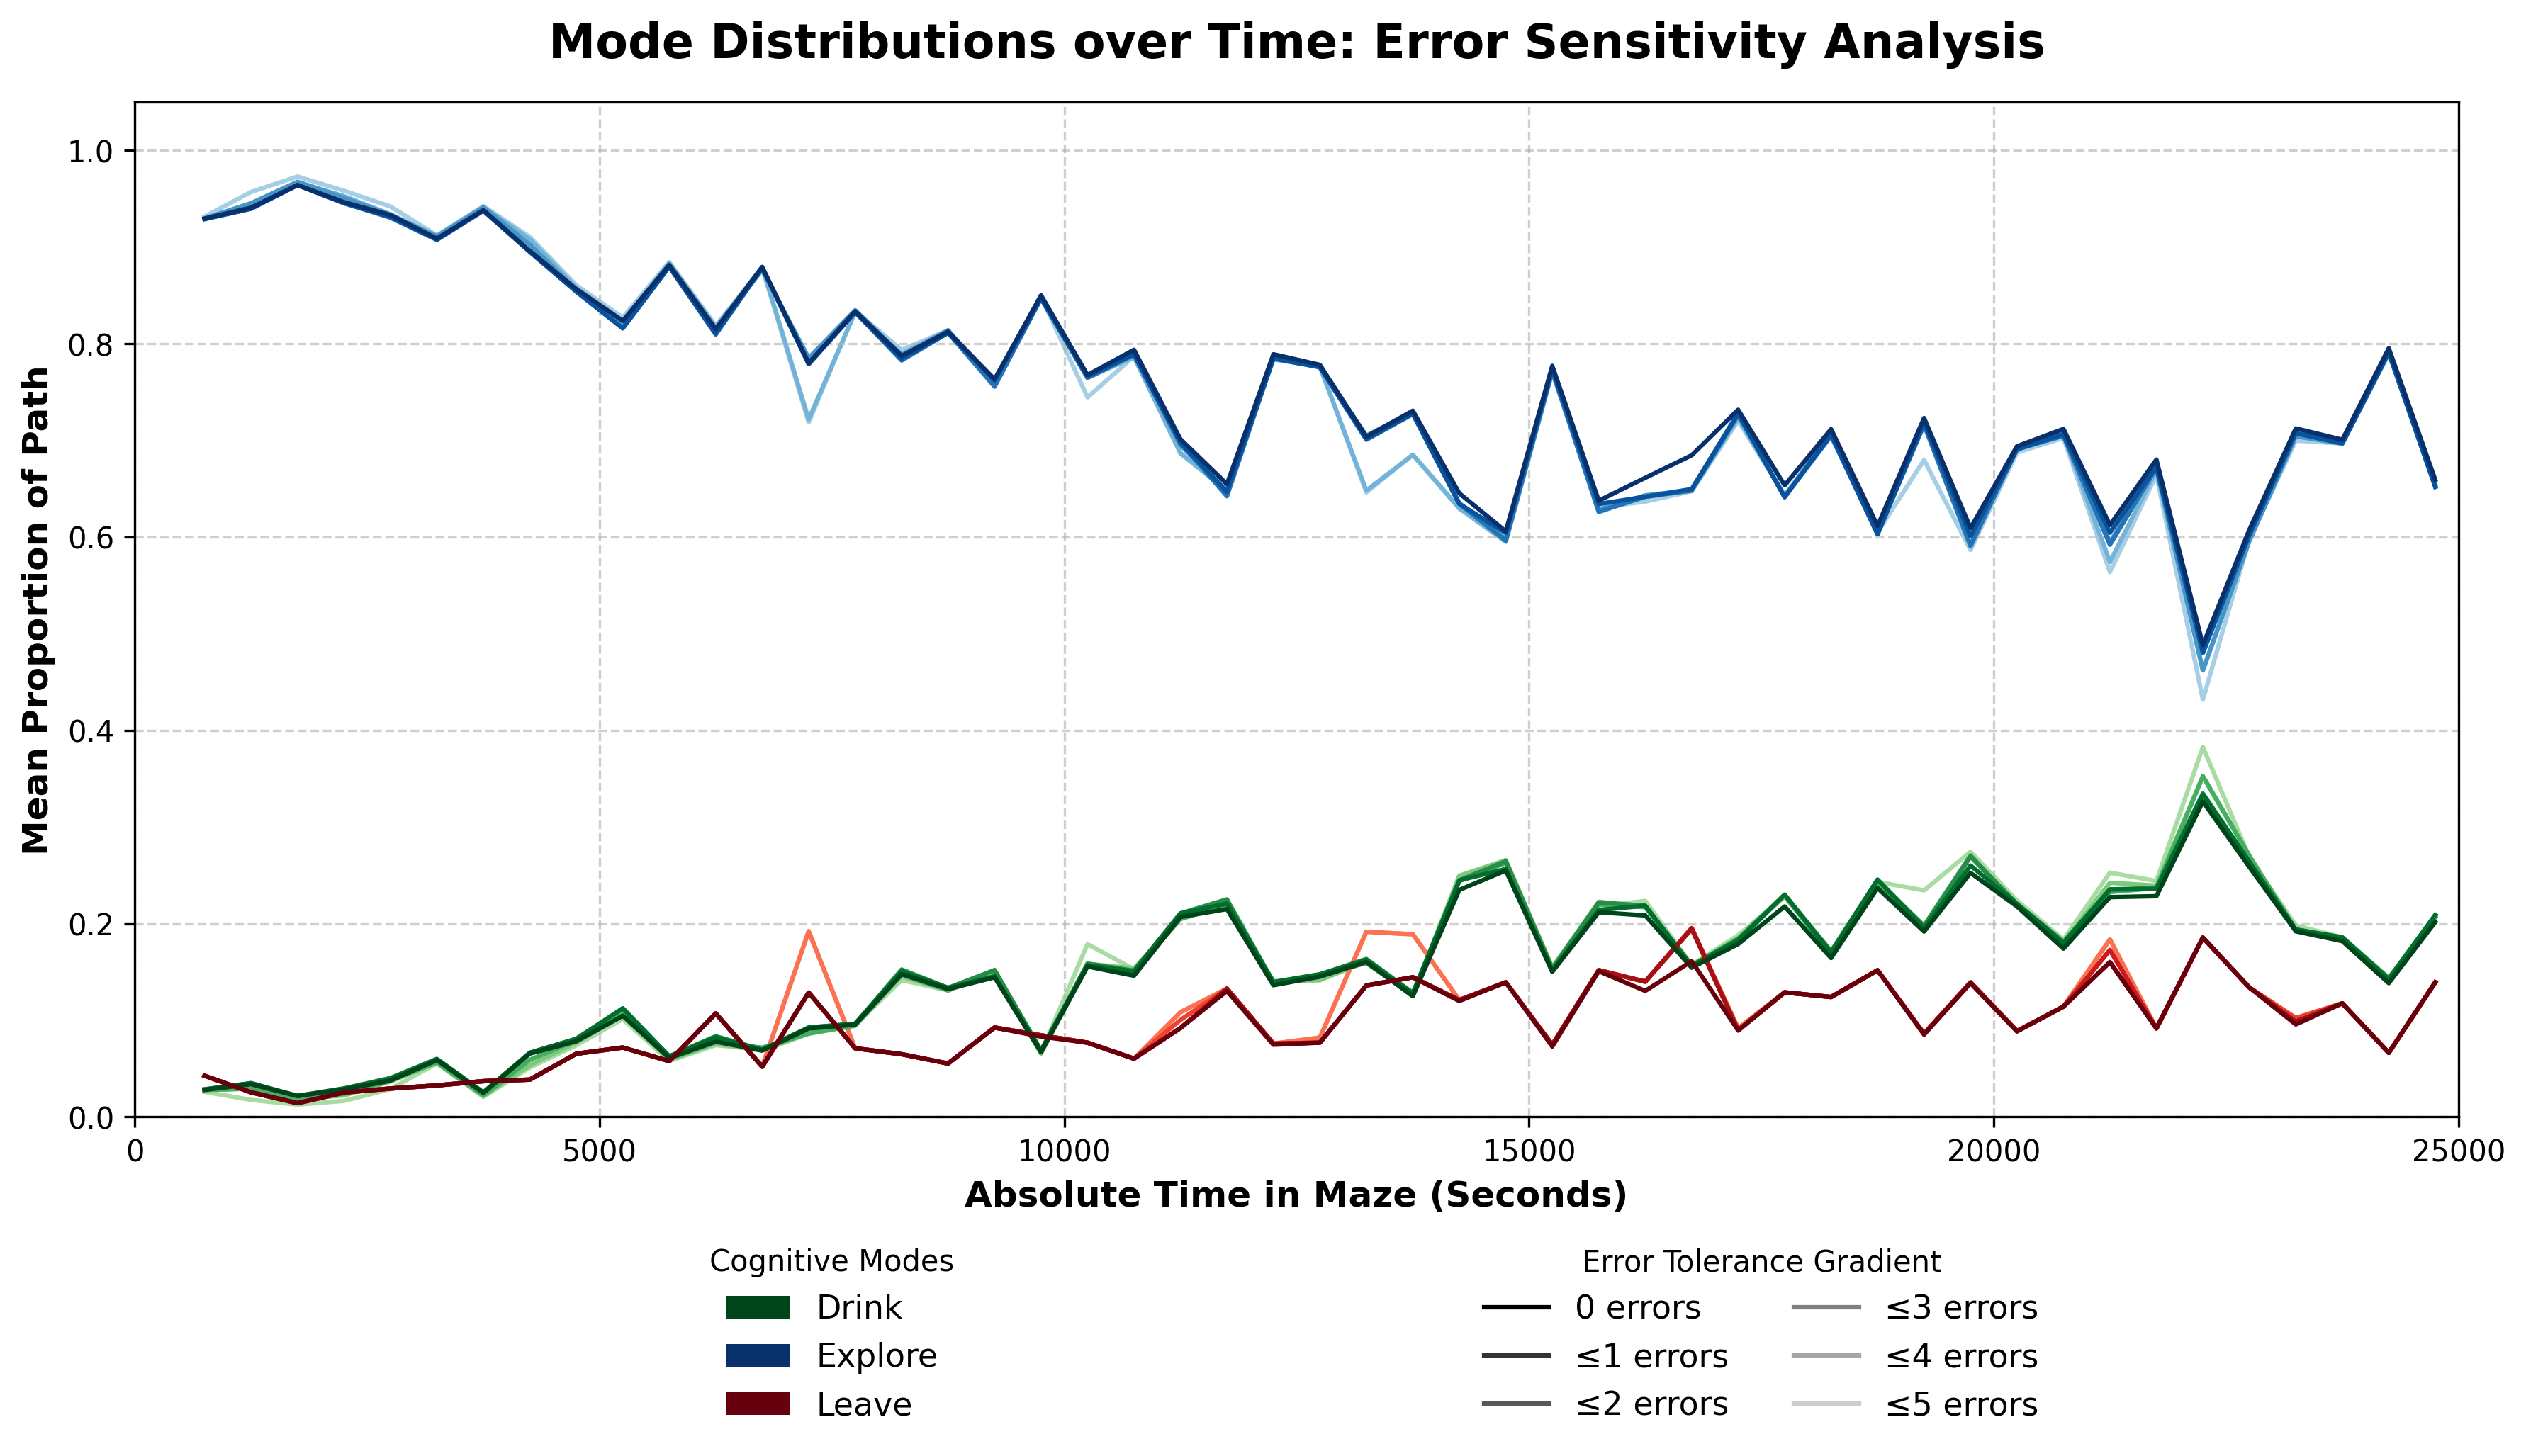
\includegraphics[width=0.48\textwidth]{figures/mode_sensitivity.png}
    \caption{\textbf{Distribution of Behavioural Modes Over Time.} Mean Behavioural mode proportion across mice, plotted over time. Tolerances shown by decreasing shade of respective mode colours for explore (blue), drink (green), leave (red)}
    \label{fig:mode_distribution}
\end{figure}

\subsection{Unrewarded Target Fixation and Short Paths}
While the three generic modes capture broad behavioural states, analysing the specific spatial distribution of unstructured \textit{explore} bouts reveals highly non-uniform tendencies. As shown in Figure \ref{fig:leaf_visits}, both the rewarded and unrewarded groups exhibit a strong baseline preference for exploring the extreme corners of the maze, followed by the outer edges, with internal nodes receiving the least attention.

However, Nodes 115 and 116 represent significant outliers to this spatial gradient. Node 116 houses the water port apparatus. Crucially, the unrewarded group exhibits a pronounced preference for investigating this specific node, despite never receiving a water reward. We propose two hypotheses for this latent target fixation: (1) residual olfactory markers left by the rewarded group despite cleaning protocols, or (2) the physical irregularity of the dry water spout acting as an inherent point of investigatory interest within an otherwise uniform maze.

\begin{figure}[htbp]
    \centering
    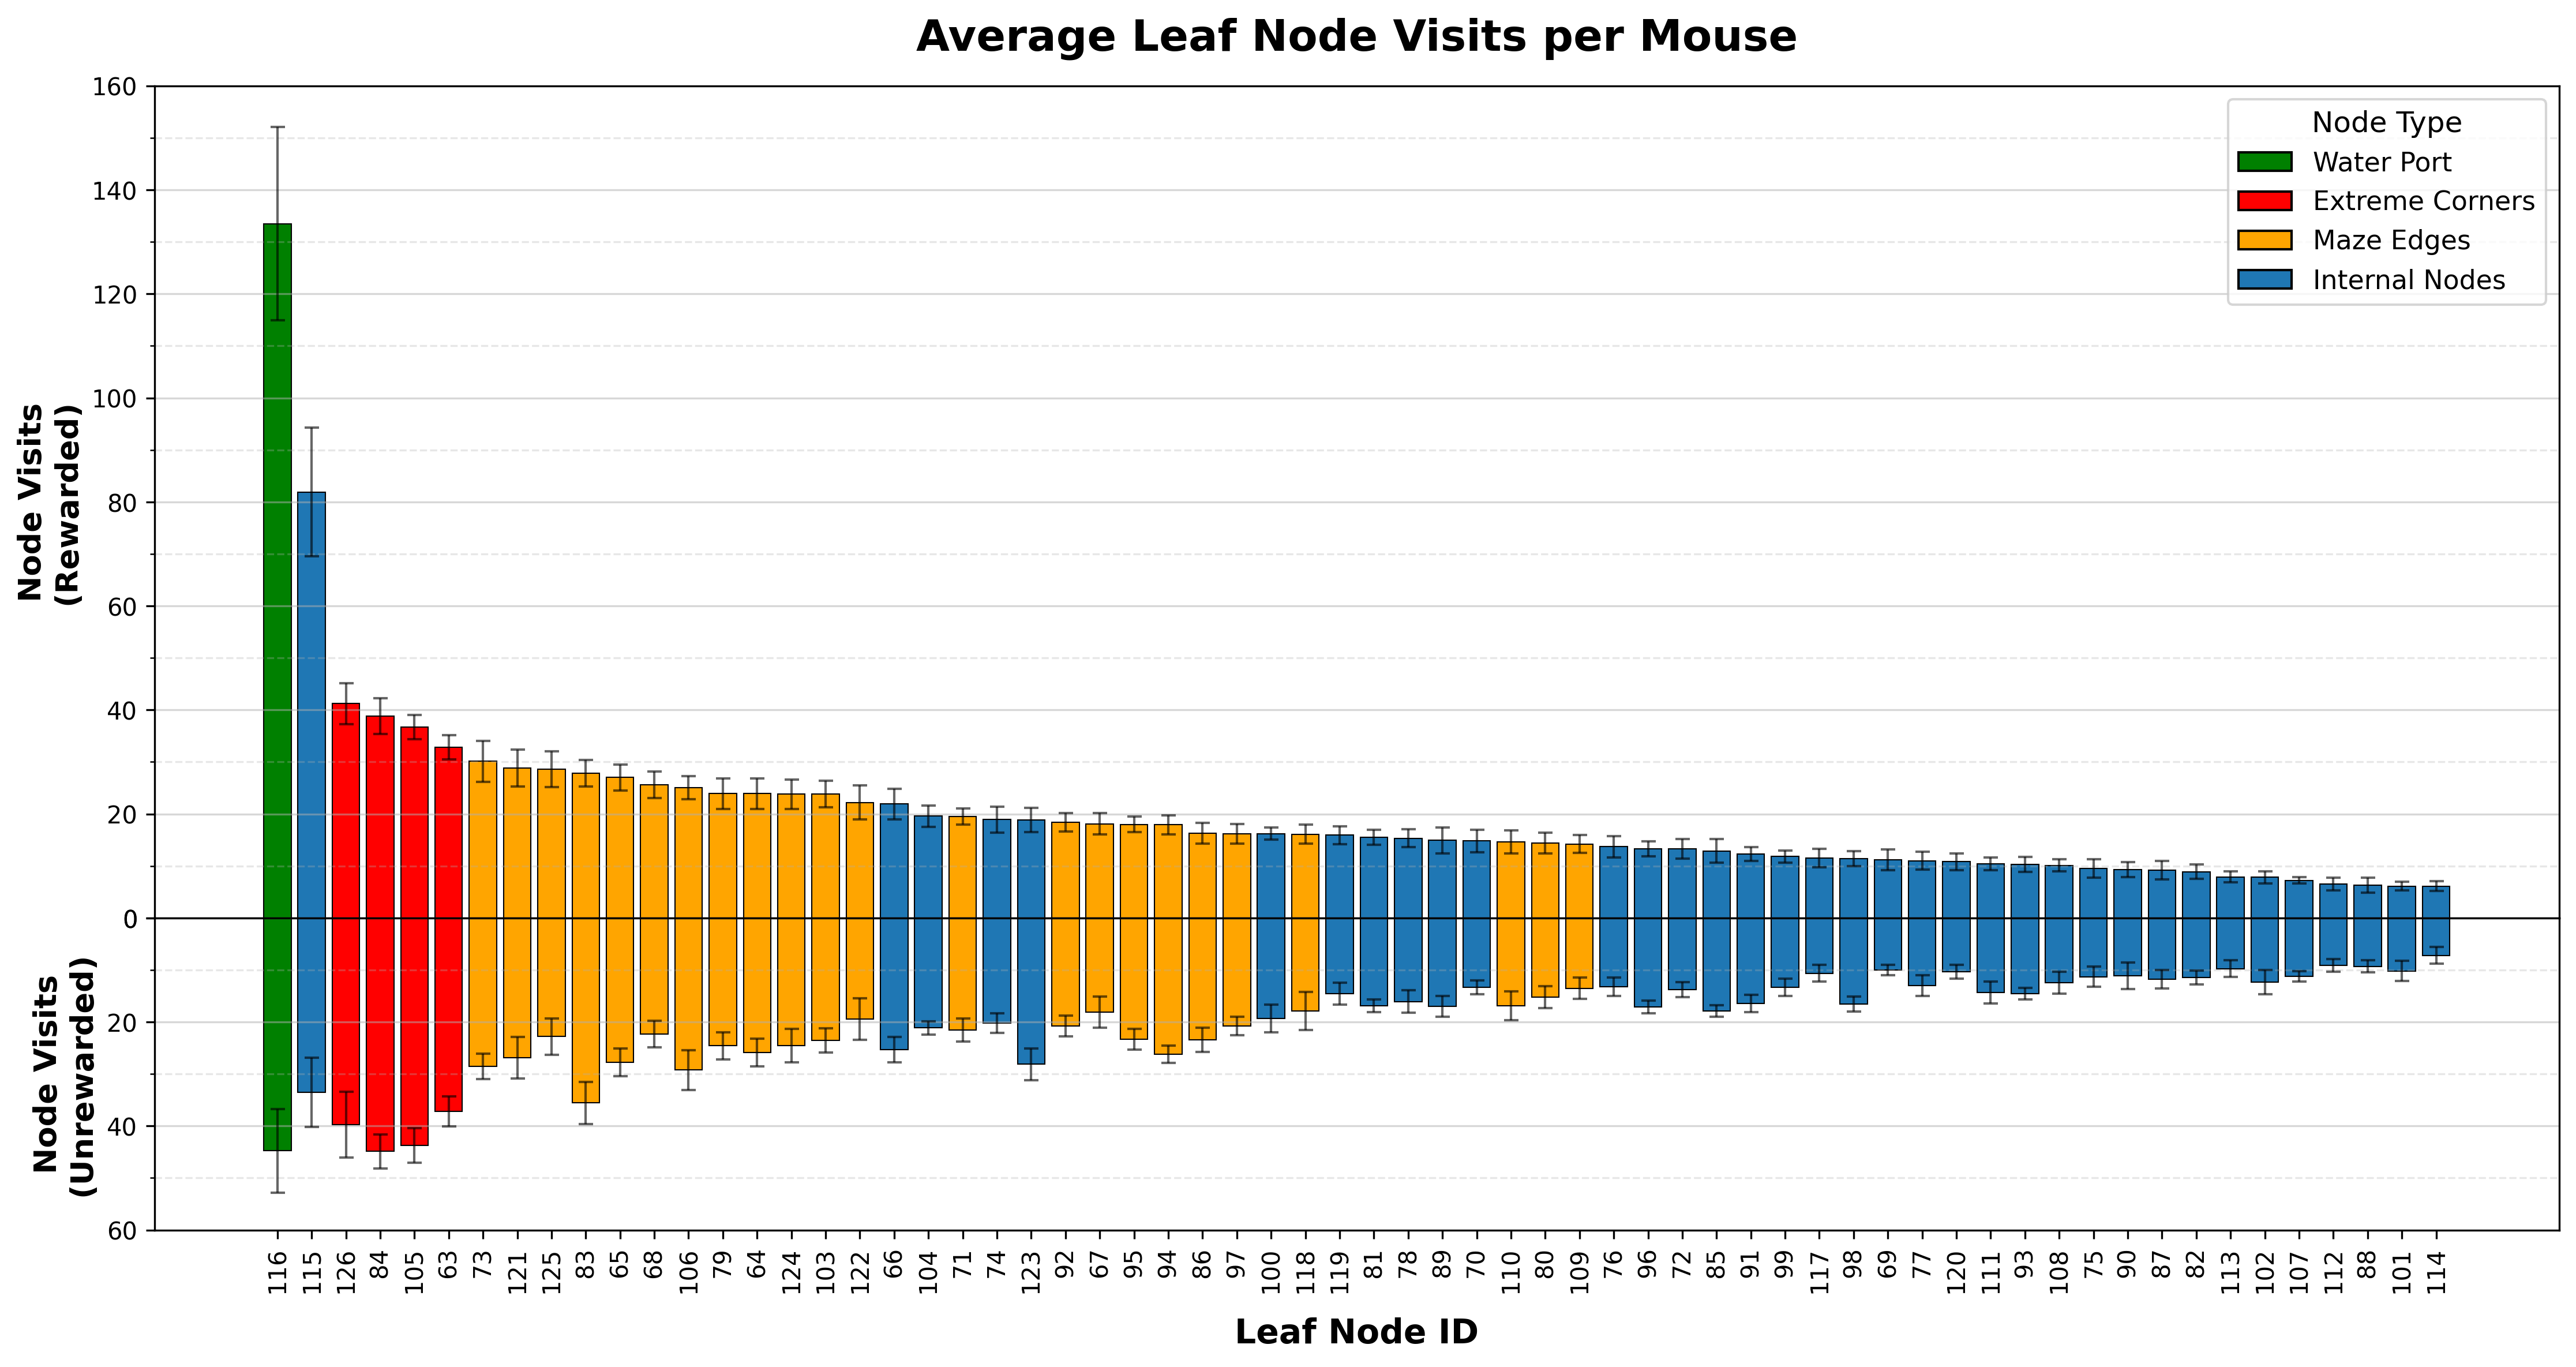
\includegraphics[width=0.5\textwidth]{figures/leaf_node_visits.png}
    \caption{\textbf{Average Leaf Node Visits.} Frequency of visits to maze leaf nodes. Both groups display a geometric preference for extreme corners (red) and edges (orange) and the water port (Node 116, green).}
    \label{fig:leaf_visits}
\end{figure}

To determine whether these visits to Node 116 were random anomalies or structured behaviour, we conducted a spatial and kinematic analysis of recurring ``short paths'', sequences of steps that mice repeat taking direct paths from home to an apex node, before returning home. Though there is no obvious pattern to these short bouts, they reveal behaviours distinct from the three modes defined. 

Our analysis of the dwell times (node duration) during these specific paths reveals a distinct kinematic signature. We partitioned these trajectories into three phases: the \textit{outbound} journey, the \textit{apex} (the deepest point of the path), and the \textit{inbound} return. As demonstrated in Figure \ref{fig:short_paths}, the mean dwell time is larger at the apex of these short paths across both groups, though still far lower than for visits to the water port.

This kinematic pausing strongly supports the hypothesis that these are not artifacts of random wandering, but rather directed investigatory ``short bouts'' or patrolling behaviours. The presence of this highly structured, goal-oriented movement within the theoretically unstructured \textit{explore} dataset suggests that future work may need to classify a fourth behavioural mode to accurately partition directed investigation from pure random exploration.

\begin{figure}[htbp]
    \centering
    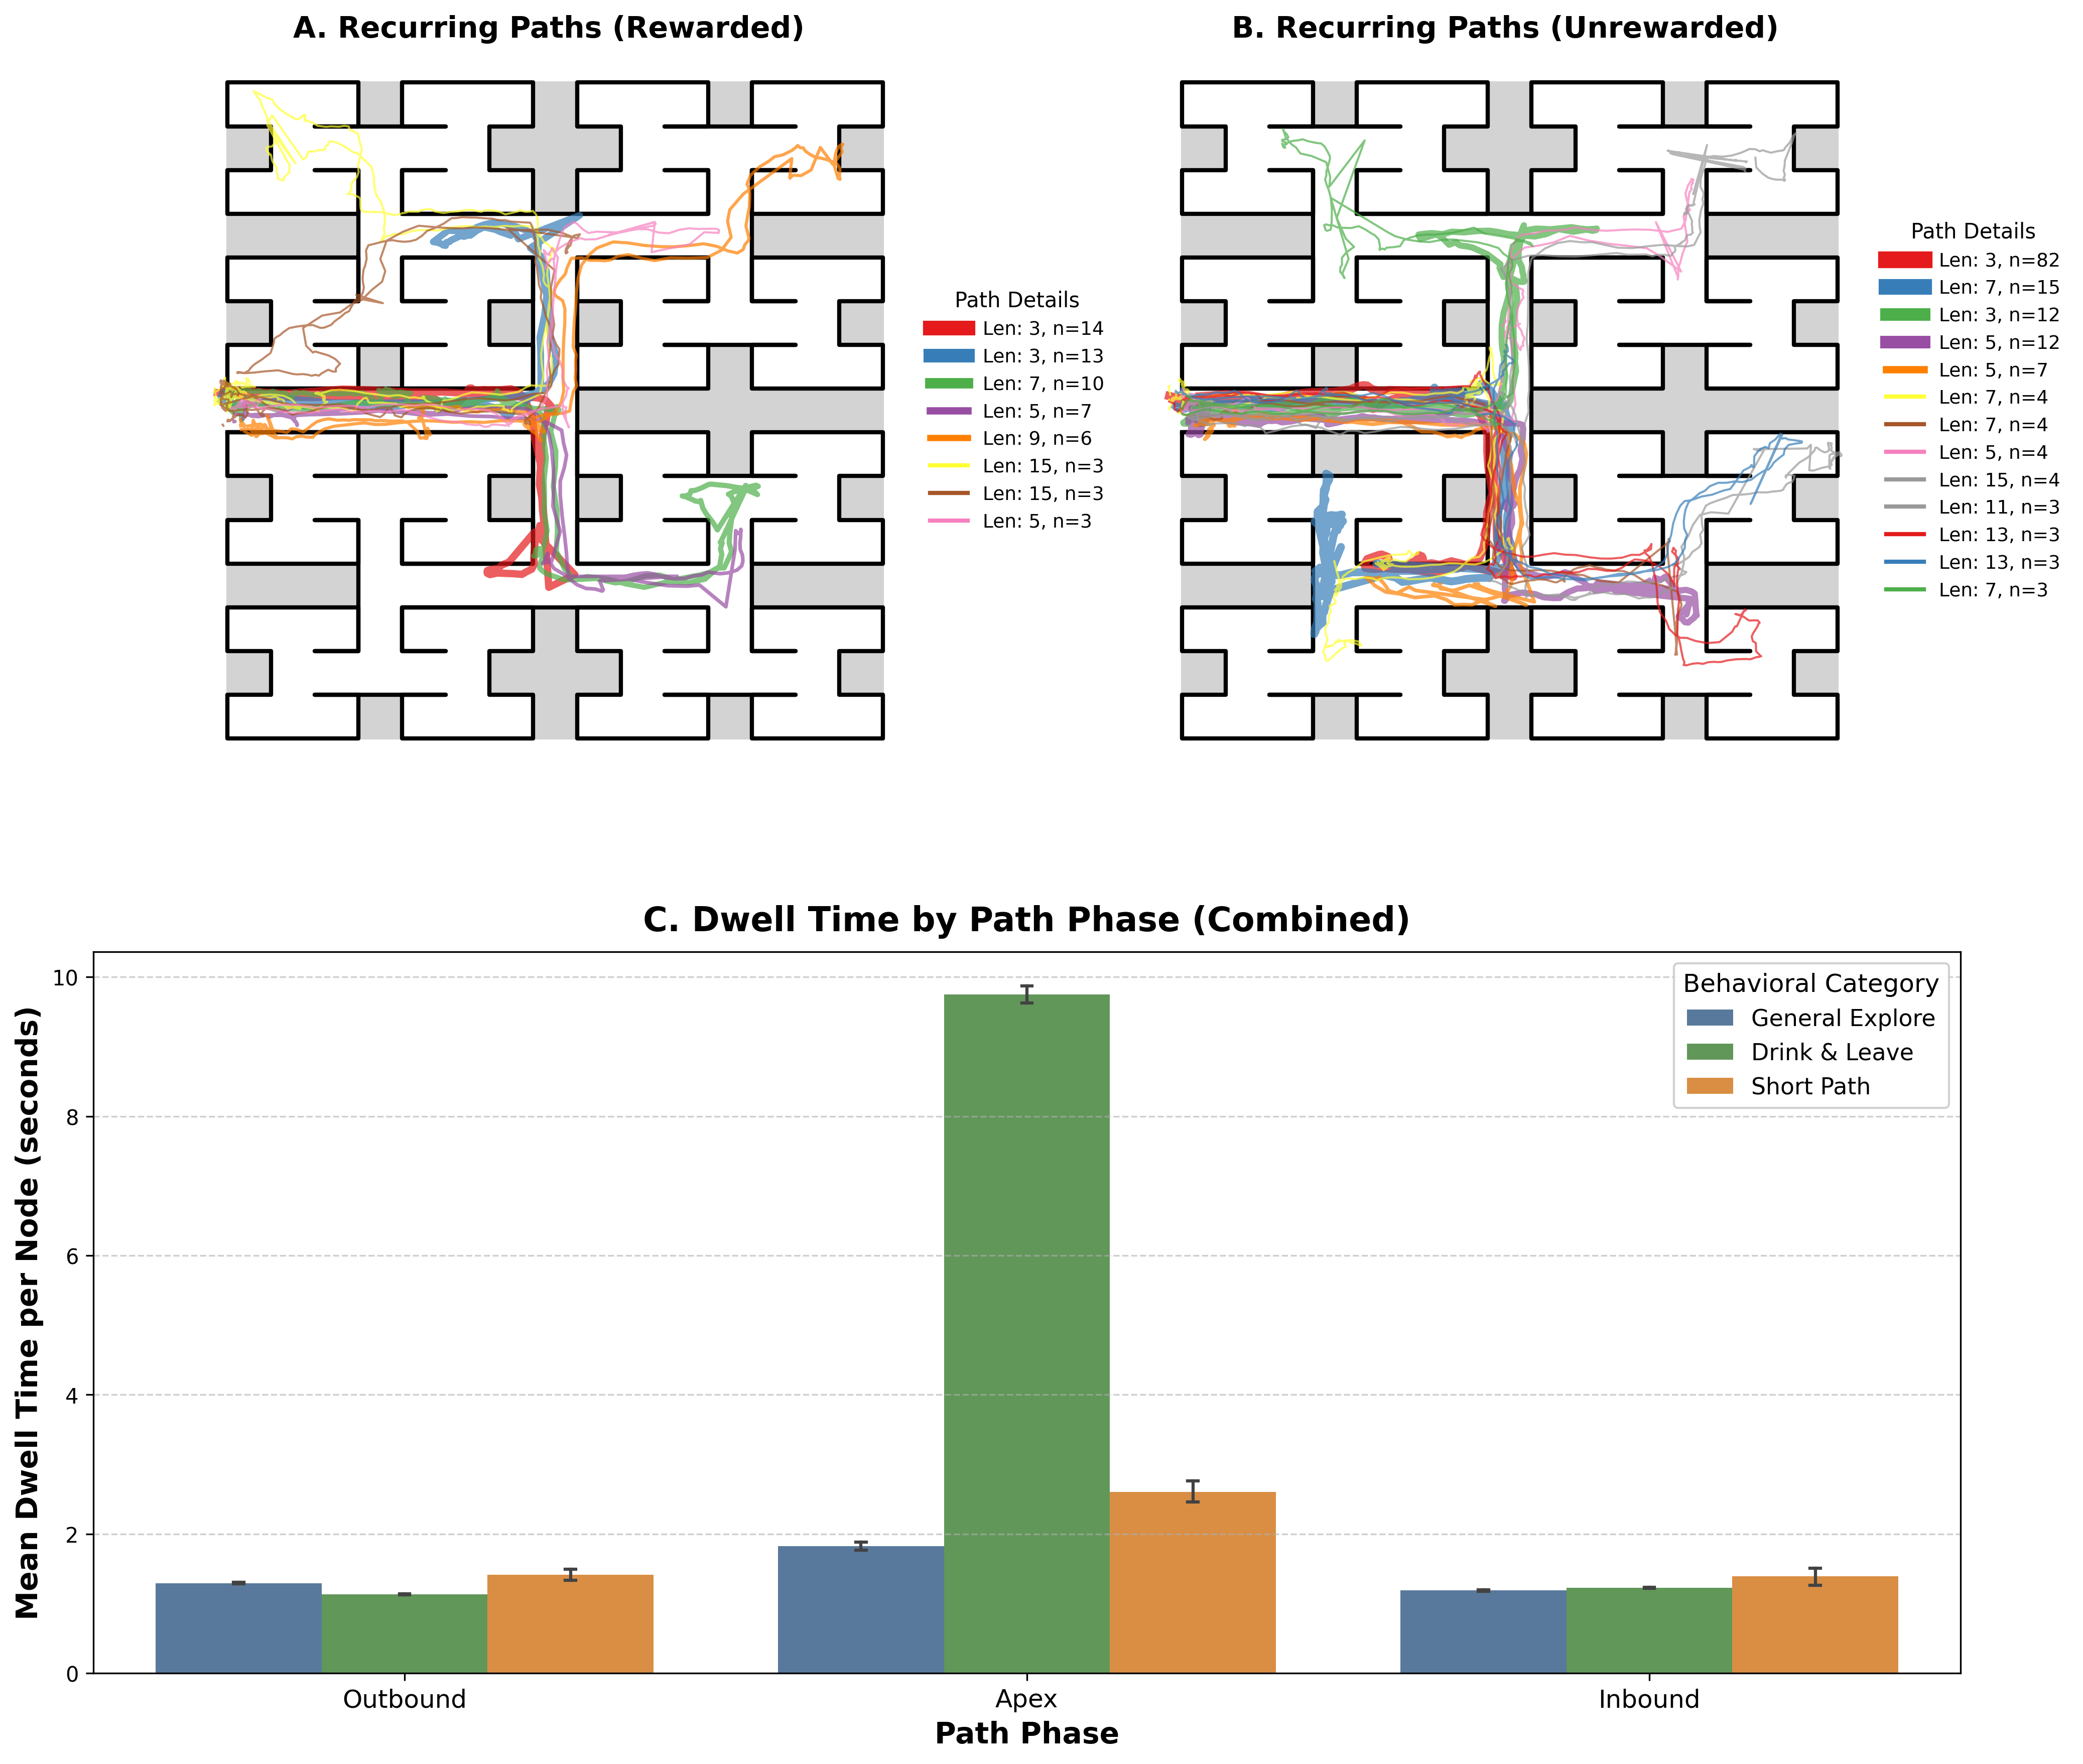
\includegraphics[width=0.5\textwidth]{figures/short_paths.png}
    \caption{\textbf{Spatial and Kinematic Profile of Recurring Short Paths.} (A, B) Analysis of node dwell times across modes and path phases. Three phases are defined: outbound, apex, and inbound. Trajectories categorised as exploration (blue), drink (green) and investigative short paths (orange).}
    \label{fig:short_paths}
\end{figure}